\chapter{Srovnání výsledků}

Odvozený model identifikovaný z rovnic v kapitole \ref{identifikovane_parametry_ch} dává do vztahu točivé momenty jednotlivých os s jejich polohami, úhlovými rychlostmi a úhlovými zrychleními (rovnice \eqref{celkova_dyn_rovnice_eq}). Tento model je dále možné použít k výpočtu celkového elektrického výkonu robotu (viz sekce \ref{el_vykon_ch}).

Pro predikci výkonu byly vypočítané momenty sil na jednotlivých osách převedeny pomocí momentových konstant motorů na efektivní hodnoty proudů protékajících jejich vinutím. Nahrazením vinutí motorů obvodem s odporem a indukčností zapojenými v sérii (obrázek \ref{schema_motoru_pic}) byly z těchto hodnot proudů vypočítány hodnoty efektivního napětí na svorkách motorů. Vynásobením hodnot napětí a proudů podle rovnice \eqref{motor_power_eq} byly vypočítány průběhy elektrických výkonů na jednotlivých osách. Celkový elektrický výkon robota je poté dán součtem všech dílčích výkonů na všech osách. 

\section{Dosažitelná přesnost modelu}
\label{dosaz_presnost_sec}
Momenty sil na jednotlivých osách v jsou nástroji TRACE vypočítány ze změřených proudů, podle vzorce \eqref{torque_current_eq}, jejich vynásobením příslušnými momentovými konstantami. Pokud by byly parametry modelu identifikovány naprosto přesně, byl by, s přihlédnutím k aproximacím a zjednodušením použitým při odvození modelu, průběh výkonu vypočítaný pomocí tohoto modelu totožný s výkonem vypočítaným z měření proudů. Výkon spočítaný pomocí těchto změřených proudů představuje maximální možnou hranici přesnosti, které je možné pomocí použitého modelu dosáhnout. 

\begin{figure}[h!]
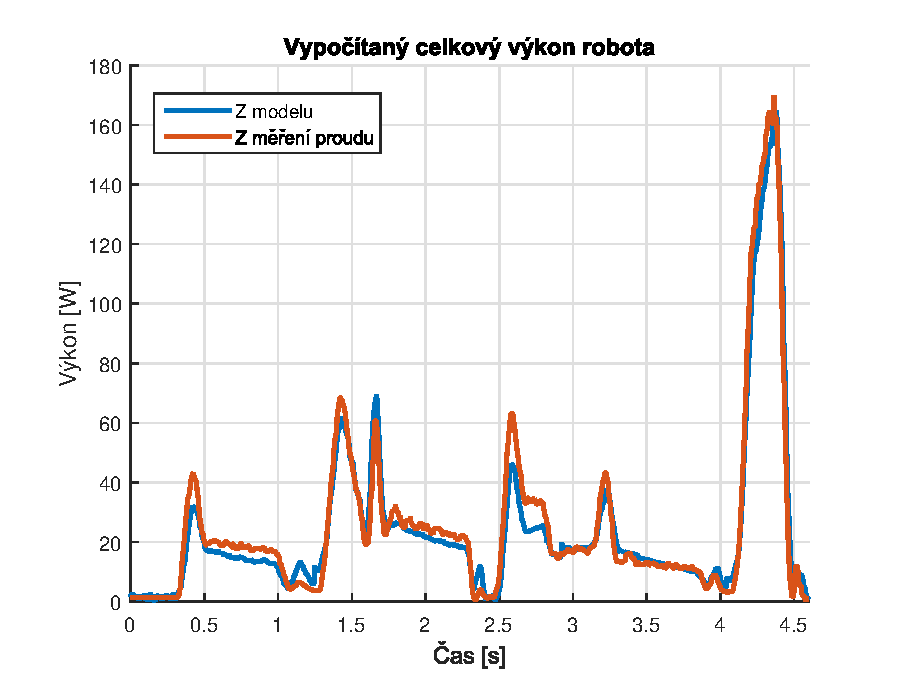
\includegraphics[width=0.9\textwidth]{model_vs_trace}
\caption{Srovnání vypočítaného výkonu z modelu a z měření proudu}
\label{model_vs_trace_pic}
\end{figure}

Na obrázku \ref{model_vs_trace_pic} je zobrazen průběh výkonu vypočítaného z modelu a z přímého měření proudů pomocí nástroje TRACE. Je patrné, že si oba průběhy poměrně odpovídají. Střední absolutní odchylka mezi oběma průběhy je 4,08 W, což odpovídá relativní střední odchylce 15,79\%. Přesnost odvozeného modelu se tedy blíží maximální možné dosažitelné přesnosti použitého modelu a jeho identifikace z rovnic systému.

\section{Srovnání modelu výkonu s reálným měřením}

Pro porovnání modelu pro výpočet výkonu s reálnými naměřenými hodnotami byla použita jiná trajektorie, než která byla použita pro jeho identifikaci. Tato testovací trajektorie byla vytvořena tak, aby se co nejvíce blížila typickým trajektoriím vyskytujícím se v průmyslových aplikacích. Byla vybrána trajektorie simulující montáž součástky A na povrch součástky B. Koncový efektor robota nejprve dojel z výchozí pozice na pozici, kde by se měl vyskytovat zásobník se součástkami A. Poté koncový efektor po obloukové trajektorii dojel na místo montáže součástky A a natočil se do požadovaného úhlu. Následně se vrátil zpět do výchozí pozice.

Při tomto pohybu robotu byl v jeho řídicím systému spuštěn nástroj TRACE zaznamenávající průběh poloh, úhlových rychlostí a úhlových zrychlení potřebný pro model výkonu. Zároveň bylo spuštěno měřicí PLC ukládající skutečný naměřený činný výkon na napájecím vedení robota. Skutečný změřený výkon je na obrázku \ref{mereni_vykonu_pic}.

\begin{figure}[h!]
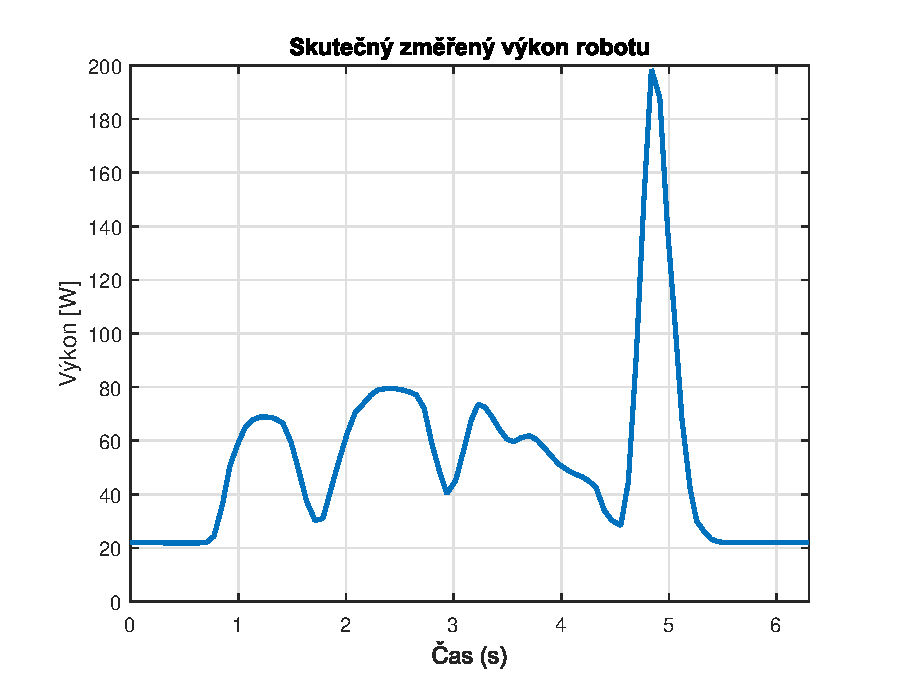
\includegraphics[width=0.9\textwidth]{mereni_vykonu}
\caption{Skutečný změřený výkon robotu}
\label{mereni_vykonu_pic}
\end{figure}

Změřené a predikované průběhy výkonu byly poté vzájemně porovnány. Aby je bylo možné mezi sebou porovnat, je nejprve nutné data upravit. První nutnou úpravou je provedení časové synchronizace mezi oběma daty. Důvodem je to, že v měřicím PLC je jiný čas než v řídicím systému robotu. Měřicí PLC zaznamenává skutečný aktuální světový čas, zatímco nástroj TRACE zaznamenává čas vztažený k okamžiku spuštění měření. 

Dále je potřeba průběhy převzorkovat, protože měřicí karta má pro měření činného výkonu vzorkovací periodu 40 ms a nástroj TRACE robotu zaznamenává data s periodou 4 ms. Nakonec byla ještě od změřených dat odečtena stálá složka výkonu, která není závislá na dynamice pohybu robotu. Z obrázku je možné určit, že hodnota stálé složky výkonu je rovna 21,9 W.

\begin{figure}[h!]
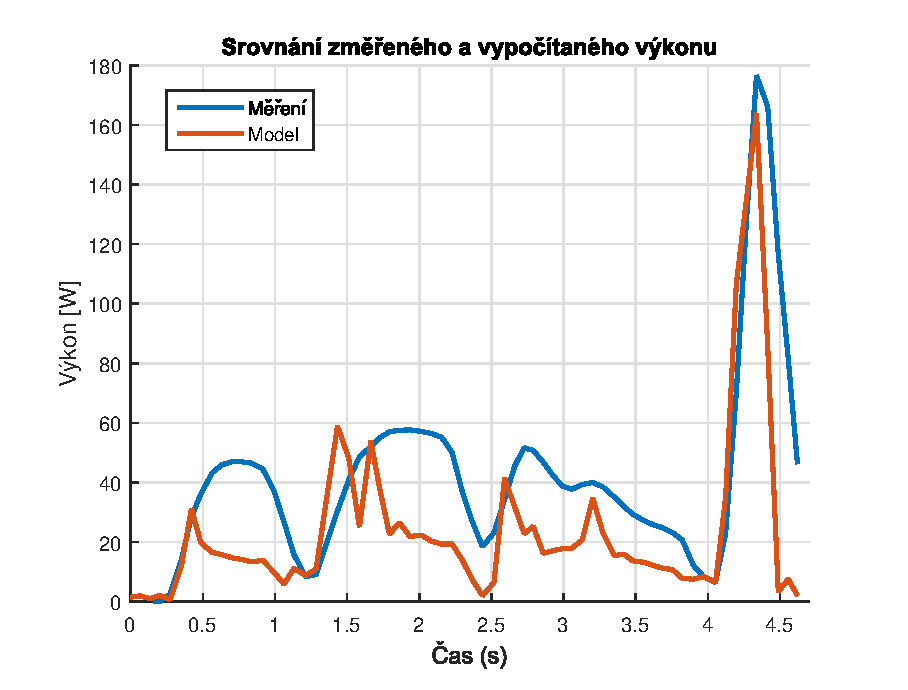
\includegraphics[width=0.9\textwidth]{model_vs_mereni}
\caption{Srovnání měření a modelu výkonu}
\label{model_vs_mereni_pic}
\end{figure}

Po provedení těchto úprav je již možné srovnat data například v MATLABu. Srovnání změřených a predikovaných výkonů z modelu je vyobrazeno na obrázku \ref{model_vs_mereni_pic}.

Porovnáním obou průběhů je patrné, že přestože oba průběhy mají podobný trend a mají minima a některá maxima ve stejných časech, nejsou tyto průběhy stejné. Průběh skutečného změřeného výkonu neobsahuje ostré špičky jako predikované hodnoty a je celkově mnohem hladší. Má také celkově vyšší amplitudu.  

\section{Analýza odchylek}
\label{analyza_odchylek_sec}

Odchylky mezi hodnotami změřeného a predikovaného výkonu mohou být způsobeny nepřesným, případně nesprávně identifikovaným, modelem nebo nesprávným měřením skutečných hodnot činného výkonu.

Z výsledků v sekci \ref{dosaz_presnost_sec} je vyplývá, že se přesnost identifikovaného modelu blíží maximální možné dosažitelné přesnosti. Nedokonale identifikované parametry modelu sice způsobí odchylku oproti měření, ta ale nebude tak velká, aby mohla odpovídat odchylce z obrázku \ref{model_vs_mereni_pic}.

Odchylka mezi měřením a modelem je tedy pravděpodobně způsobena nesprávným měřením výkonu. Jednou z možností je nepřesnost měřicího systému s měřicí kartou WAGO-I/O-SYSTEM 750. Tento měřicí systém byl vytvořen Ing. Vojtěchem Pavlíkem v rámci jeho diplomové práce \cite{vojtech_pavlik}. Použitá měřicí karta byla nakonfigurována v souladu s její dokumentací a celý systém otestován. Následně byl tento systém úspěšně použit v průmyslovém prostředí. Je rovněž možné vyloučit nepřesnost měření proudu v řídicím systému robotu KUKA KR5 Arc. Řídicí systém robotu ovládá otáčení motorů regulací proudu protékajícího jejich vinutí. Nepřesnost měření proudu by tedy měla za následek i nepřesnost v řízení pohybu robotu. 

Druhou možností je nesprávný způsob měření. Měření skutečného výkonu je prováděno způsobem popsaným v sekci \ref{mereni_el_vykonu_sec}. Reálný výkon je měřen přímo na napájecím vedení celého robotického systému. Výkon predikovaný odvozeným modelem je ale vztažen k elektrickému výkonu ve vinutí motorů robotu. 

Motory robotu jsou řízeny frekvenčními měniči umístěnými v rozvaděči jeho řídicího systému. Frekvenční měniče jsou systémy schopné nezávisle řídit frekvenci a amplitudu elektrického proudu, který generují. Tyto systémy působí jako samostatné zdroje elektrické energie. 

V dokumentaci robotu KUKA KR5 Arc nejsou žádné informace o použitých frekvenčních měničích pohánějících servomotory robotu. Moderní frekvenční měniče jsou komplexní samostatné systémy, často s vlastními řídicími jednotkami a složitou elektronikou. Jsou navrhovány tak, aby byly schopny generovat vysoké výstupní výkony a nedocházelo k velkému poklesu napájecího napětí motorů při krátkých proudových impulsech. Dále bývá jejich řídící logika navržena tak, aby eliminovala příliš vysoké proudové špičky za účelem snížení zátěže mechanických částí motoru.

Na obrázku \ref{fazovy_posun_pic} je průběh fázového posunu mezi napětím a proudem na napájecím vedení robotického systému při vykonávání určité trajektorie. Tento fázový posun byl vypočítán z měření činného a zdánlivého výkonu. 

\begin{figure}[h!]
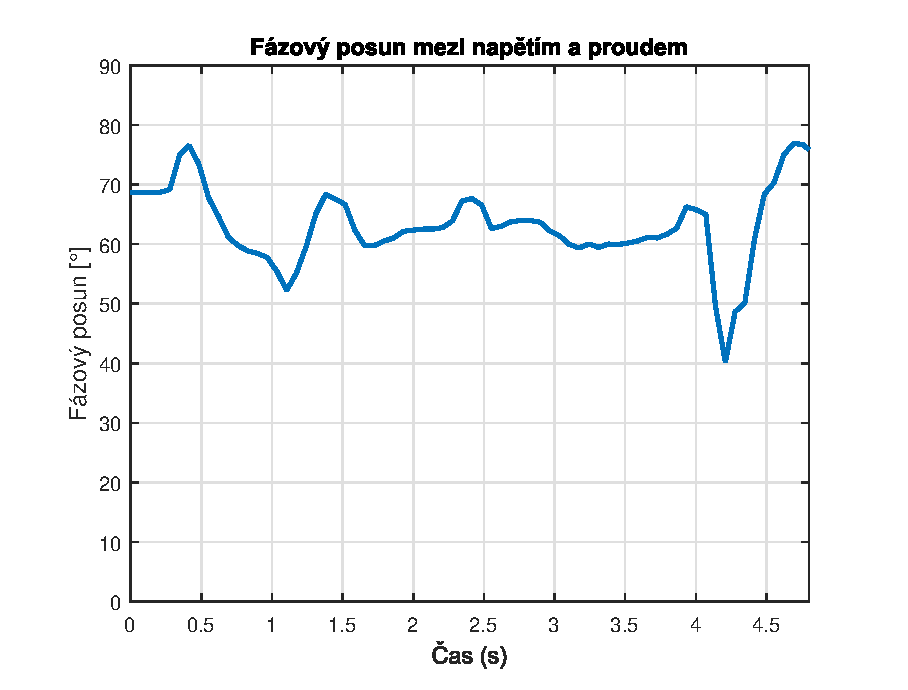
\includegraphics[width=0.9\textwidth]{fazovy_posun}
\caption{Fázový posun mezi napětím a proudem na napájecím vedení robotu}
\label{fazovy_posun_pic}
\end{figure}

Z průběhu je patrné, že se fázový posun mezi napětím a proudem během během pohybu robotu velmi mění. Elektroniku frekvenčních měničů proto není možné nahradit jednoduchým modelem s pasivními elektronickými prvky.  

Pro srovnání je na obrázku \ref{proudy_pic} porovnání celkového efektivního proudu změřeného měřicí kartou WAGO-I/O-SYSTEM 750 a celkového efektivního proudu změřeného nástrojem TRACE robotu. Celkový proud měřený nástrojem TRACE je dán jako součet absolutních hodnot proudů ve všech motorech.

\begin{figure}[h!]
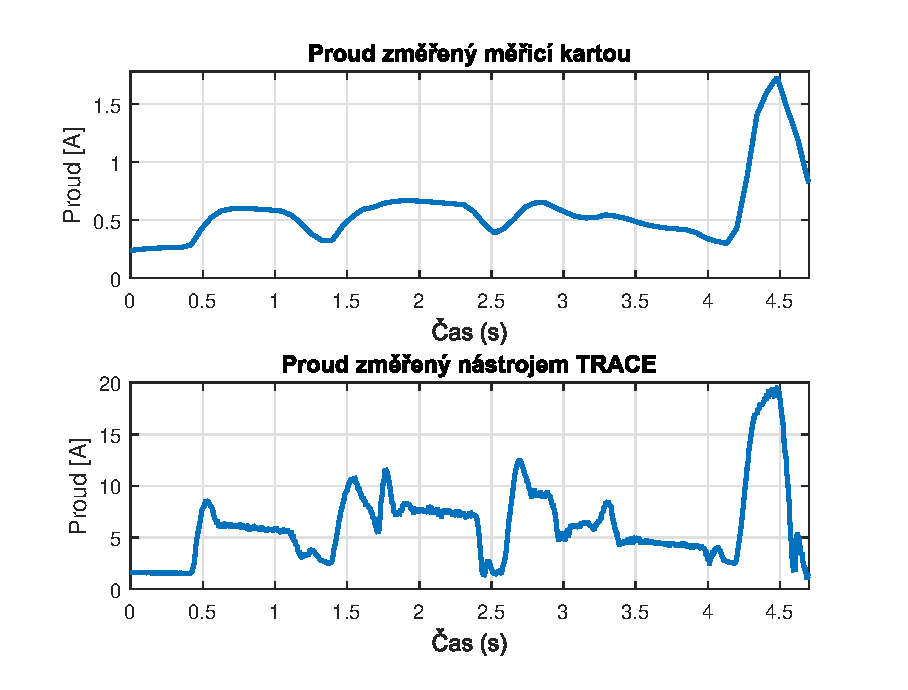
\includegraphics[width=1\textwidth]{proudy}
\caption{Srovnání celkových změřených proudů}
\label{proudy_pic}
\end{figure}

Z grafů je patrné, že průběh obou proudů je velmi podobný. Kromě vyšší amplitudy má proud změřený nástrojem TRACE mnohem ostřejší hrany a proudové špičky. Protože frekvenční měniče nejsou ideálními zdroji elektrické energie, je možné předpokládat, že při tak vysokých, ostrých a rychlých proudových špičkách může docházet k poklesu napájecího napětí motorů. Výsledný elektrický výkon by poté tak ostré špičky neobsahoval. Toto tvrzení ale není možné ověřit měřením, protože nástroj TRACE neumožňuje měření napájecích napětí motorů.

\newpage

Dále je možné předpokládat, že v rozvaděči celého robotického systému jsou kromě frekvenčních měničů také další elektronické prvky sloužící ke stabilizaci napájení jednotlivých jeho částí. 

Z těchto důvodů by pro snížení odchylky mezi změřeným a predikovaným výkonem bylo potřeba model výkonu robotu doplnit o modely frekvenčních měničů napájejících motory robotu a dalších prvků v jeho rozvaděči. Druhou možností je upravit způsob měření reálného výkonu tak, aby měřil výkony přímo na motorech robotu. Jednalo by se ale o intrusivní měření, kterému se tato práce snaží vyhnout.